\section{Design and implementation}

The implementation was created using Futhark, Futhark is a functional language which focuses on compiling effecient parallel code.
Futhark comes with some limitations, one being that arrays cannot be irregular or contain functions.
If this limitation was not there, it would be easy to make an array of the functions for each layer and then use a \texttt{fold}-like operation for the forward propagation.

\subsection{Design}

The design idea was to implement each layer as a module that could calculate the forward propagation and update the weights given a gradient.
The idea of combining layers into a network was part of the design early on.
This meant that there needed to be a way to store the forward propagation function and the weights of the entire network.
It was also important that the weights could be given as a single argument to the network, since that would be used for the automatic differentiation function \texttt{vjp}. The type of \texttt{vjp} can be seen in the following listing.
\begin{lstlisting}
val vjp 'a 'b : (f: a -> b) -> (x: a) -> (y': b) -> a
\end{lstlisting}

This then lead to the idea of storing the forward function and weights in a record like the following. It should also be important to store a function that can apply the gradient to the weights, in this project it is called \texttt{apply\_optimize}.

\begin{lstlisting}
type^ nn_type 'input 'output 'current_weight 'rest_weights = {
  forward: input -> (current_weight, rest_weights) -> output,
  apply_optimize: (current_weight, rest_weights) -> (current_weight, rest_weights) -> (current_weight, rest_weights),
  weights: (current_weight, rest_weights)
}
\end{lstlisting}

This means that it is easy to add a new layer to the network by simply composing the \texttt{forward} function, \texttt{apply\_optimize} function and adding the weights of the current layer to the \texttt{current\_weight} part of the \texttt{weights} tuple.
It also means it is easy to call the forward propagation of the network with some input.

In \autoref{lst:add_layer} it can be seen how layers can be composed in a simplified way.

\begin{lstlisting}[caption=A simplified version of adding a layer to a network, label={lst:add_layer}]
def add_layer (layer) (network) =
  let {
    apply_optimize = layer_apply_optimize,
    forward = layer_forward,
    weights = layer_weights,
  } = layer
  let { apply_optimize, weights, forward } = network
  let new_forward = (\input (cw, rw) -> layer_forward (forward input rw) cw)
  let new_apply_optimize = (\(cw, rw) (cg, rg) -> (layer_apply_optimize cw cg, apply_optimize rw rg)
  in {
    weights = (layer_weights, weights),
    apply_optimize = new_apply_optimize,
    forward = new_forward
  }
\end{lstlisting}

To add layers to a network, the network needs to be initialized, the way the network is initialized is by setting the \texttt{forward} and \texttt{apply\_optimize} functions as an identity functions of the input and keep the weights as two empty tuples \texttt{((), ())))}.

It is also important that layers follow the same type, so they work with the \texttt{add\_layer} function, the type of layers can be seen in the following listing.

\begin{lstlisting}
type^ layer_fwd_type 'options 'layer_input 'wb 'out = options -> layer_input -> wb -> out
type^ layer_apply_optimize_type 't 'apply 'options 'weights = options -> apply -> weights -> weights -> weights
type^ layer_type 't 'options 'layer_input 'wb 'shape 'out = {
  forward: layer_fwd_type options layer_input wb out,
  apply_optimize: layer_apply_optimize_type t options wb,
  options: options,
  weights: wb,
}
\end{lstlisting}

Here \texttt{layer\_fwd\_type} is the type of the forward function inside a layer. In \texttt{layer\_type} there is also a field for \texttt{options}, this can be different for different layer type, but can as an example contain information about strides or padding.

\subsection{Interface}

One part of the design was to make the interface as easy to use as possible, this was attempted by adding a \texttt{shape} field for the neural network type. The intention with this field was that it could be used to define the input shape of the next layer, in such a way that the user could avoid having to manually type in the output sizes of some layers. However due to limitations of Futhark it was not possible to use a field in a record to define size types. The intended way to this would be something like the following listing.

\begin{lstlisting}[caption=the \texttt{add\_layer} function but with an added field \texttt{shape}.]
def add_layer (layer) (network) =
  let {
    apply_optimize = layer_apply_optimize,
    forward = layer_forward,
    weights = layer_weights,
    shape = layer_shape,
  } = layer
  let { apply_optimize, weights, forward, shape } = network
  let new_forward = (\input (cw, rw) -> layer_forward (forward input rw) cw)
  let new_apply_optimize = (\(cw, rw) (cg, rg) -> (layer_apply_optimize cw cg, apply_optimize rw rg)
  in {
    weights = (layer_weights, weights),
    apply_optimize = new_apply_optimize,
    forward = new_forward,
    shape = layer_shape
  }
\end{lstlisting}

Here the \texttt{shape} field could define the output shape of the network and we could destructure the layer in the parameters and use the shape values in the return type.

The interface for the layers will be described more in \autoref{sub:layers}

\subsection{Library structure}

In this section an overview of the library structure will be given.

The largest part of the library is contained within one module with multiple submobules, the reason for this is that it provides a nice interface and the user of the library would not have to import each feature that they need.
The idea is that the user can import \texttt{neural-network/neural-network} as a module that can be called \texttt{nn}, and then access close to the entire library.

Layers are each defined in their own module, this makes sense since there are much functionality and many components that should only be used in one place, so naturally it makes sense to separate it it.
Layers can be accessed by the user in \texttt{nn.layers} and are defined in the \texttt{layers/} directory.

\subsection{Activation functions}

Activation functions in this implementation is simple and its type is represented as the following

\begin{lstlisting}[caption=The type definition of activation functions., label={lst:activation_type}]
type^ activation_type 't = (n: i64) -> [n]t -> [n]t
\end{lstlisting}

The reason that \texttt{n} needs to be given as an argument is that otherwise Futhark might try to generalize \texttt{n}, which would result in compilation errors when having multiple layers of different output sizes.

The activation functions can be accessed by the user in \texttt{nn.activation}.

The user can also define their own activation functions and use them as long as they follow the type described in \autoref{lst:activation_type}.

\subsection{Loss functions}

The loss functions are used in a different way than activation functions. A loss function of the network can be defined be using the function \texttt{nn.make\_loss}, this function should return a function that takes an array of inputs and an array of labels and return an array of errors. The loss functions type is defined as the following

\begin{lstlisting}
type^ loss_type 'input 'labels 't = [k]input -> [k]labels -> [k]t
\end{lstlisting}

The user can also define their own loss functions if the library does not provide it. The user defined loss function can also be given to the \texttt{nn.make\_loss} function.

\subsection{Optimizers}

Optimizers are the modules that perform the back propagation of the network.
This has been separated as its own module type to allow for new or future implementations of optimizers.

There is implemented one optimizer, which performs gradient descent this module is called \texttt{sgd} and can be accessed in \texttt{nn.optim.sgd}.

\subsection{Layers}%
\label{sub:layers}
% Layers
% Unit tests
% Interface

There are implemeted three types of layers, the fully connected layer (\autoref{ssub:impl_fully_connected}), max pooling (\autoref{ssub:impl_max_pool}) and convolutional (\autoref{ssub:impl_conv}).
To make sure the implementation works with different layers that out put different shapes and dimensions, there is also implemented a layer that transforms the output of the previous layer to the shape the user likes. This layer will be described in \autoref{ssub:impl_dimension}.

In the implementation a few shorthand functions have been added to easily add basic layers to the network, these will be described in the following subsubsections.

\subsubsection{Fully connected}%
\label{ssub:impl_fully_connected}

The fully connected layer is initialized with the function \texttt{nn.layers.linear.init} which is a function that takes \texttt{m} and \texttt{n} as its input and output size, an activation function and a seed for initializing weights.
The bias and weights can be set by the user by using the functions \texttt{nn.layers.linear.set\_bias} and \texttt{nn.layers.linear.set\_weights}, this might be useful if the user already trained a network and wants to set teh weights and bias to use the trained network without training it again.

A shorthand function for adding a linear layer ot a network is by using the functions \texttt{nn.linear}, this function takes a parameter \texttt{n} which is the output size, an activation function and the network the linear layer should be added to. This function is handy since it is very easy to compose multiple layers, with very little code. Here is an example

\begin{lstlisting}
nn.init_1d 5 1
|> nn.linear 8 (nn.activation.relu)
|> nn.linear 6 (nn.activation.relu)
\end{lstlisting}

This makes sure that the user does not need to manually input the input sizes for each layer which could lead to errors if the user is not careful.
To illustrate the difference it makes the following example shows the exact same network, but by using the \texttt{add\_layer} function and initializing each layer manually.

\begin{lstlisting}
let net = nn.init_1d 5 1
let net = nn.add_layer (nn.layers.linear.init 5 8 (nn.activation.relu) net.seed) net
|> nn.add_layer (nn.layers.linear.init 8 6 (nn.activation.relu) net.seed)
\end{lstlisting}

However in the first example, the user will not be able to set the weights and bias, but they will in the second example.

In terms of performance the operation is basically just a matrix-vector multiplication, recall the formula from \autoref{sub:Fully connected layer}
$$\bm{y} = \bm{\sigma} \left( \bm{b} + \bm{W} \bm{x} \right)$$
But since the implementation works on batches or multiple inputs, this can pratically be turned into a matrix-matrix multiplication
$$\bm{Y} = \bm{\sigma} \left( \bm{B} + \bm{W} \bm{X} \right)$$
Where $\bm{Y}$ is a matrix of outputs built from the outputs $\bm{y}$ and $\bm{X}$ is a matrix of inputs built from the outputs $\bm{x}$. $\bm{B}$ would then be the bias vector $\bm{b}$ copied $k$ times to match the size $\bm{Y}$.
Now $\bm{\sigma}$ should only be applied on each column vector in the matrix instead of the entire matrix.
This could give better performance since there are ways to optimize matrix-matrix multiplication a lot.
In an implementation of this, $\bm{b}$ could probably just be added to $\bm{WX}$ by using a \texttt{map}-like function.
However in the current state of the implementation this is not implemented, but should be very easy to implement.

\subsubsection{Max pooling}
\label{ssub:impl_max_pool}

The max pooling layer is straight forward to implement, for each slice of the input the maximum element should be found.
In regard to the interface, the intention was to let the user define the window width and height.
However due to Futhark's limitation on return sizes it made more sense to let the user give the output sizes instead.
This layer can be instantiated with different dimensions with \texttt{init\_1d} and \texttt{init\_2d}.

The \texttt{init\_2d} function takes \texttt{output\_m} and \texttt{output\_n}, which is the size of the output.
The window sizes is then calculated by an integer division which can be seen in the following listing.
\begin{lstlisting}
let window_width = m / output_m
let window_height = n / output_n
\end{lstlisting}
Where \texttt{m} and \texttt{n} are the input sizes.

\subsubsection{Convolutional}
\label{ssub:impl_conv}

The current implementation of the convolutional layer is very simple. \autoref{lst:conv_forward} shows a simplified way of how the convolutional layer works for a two-dimensional input.

\begin{lstlisting}[label={lst:conv_forward}, caption=A simplified forward function for the 2d convolutional layer. Where \texttt{a} and \texttt{b} are the sizes of the kernel.]
let c = a * b
map (\batch ->
  map2 (\filter_out_channel bias_channel ->
    map (\x ->
      map (\y ->
        map2 (\in_channel filter_in_channel -> -- the current in channel
          let input_slice = in_channel[x:x+a,y:y+b]
          let flat_slice = flatten_to c input_slice
          let flat_filter = flatten_to c filter_in_channel
          in lalg.dotprod flat_slice flat_filter
        ) batch filter_out_channel
        |> R.(sum)
        |> (+bias_channel)
      ) ys
    ) xs
  ) filter_weights bias
  |> flatten_3d batch
  |> activation_func (out_channels * output_m * output_n)
  |> unflatten_3d out_channels output_m output_n
) input
\end{lstlisting}

The \texttt{filter\_weights} is an array of the kernels where each kernel is three dimensional (\texttt{out\_channels}, x, y).
\texttt{xs} and \texttt{ys} are arrays that are generated by \texttt{iota}, an example can be seen in the following listing

\begin{lstlisting}
let xs = iota output_m -- m - a + 1
\end{lstlisting}

Since Futhark cannot return size types based on arithmetic for example $m - a + 1$, that means the user has to provide the output size, in this example \texttt{output\_m}.

The convolutional layer can be instantiated with multiple functions, there is \texttt{init\_1d} and \texttt{init\_2d}, each depending on the shape of the input.
\texttt{init\_1d} instantiates a layer that takes a two-dimensional array as input, where the first dimension is the channels.
\texttt{init\_1d} is instantiated with the follwing parameters
\begin{itemize}
    \item \texttt{output\_n}: the output size of the input.
    \item \texttt{in\_channels}: the number of input channels of the input.
    \item \texttt{out\_channels}: the number of channels the output should have, this also means how many kernels the layer should have.
    \item \texttt{kernel\_sz}: The size of the one-dimensional kernel.
    \item \texttt{activation\_func}: The activation function for the layer.
    \item \texttt{seed}: The seed to use for initializing weights.
\end{itemize}
For \texttt{init\_2d} it is the same as \texttt{init\_1d}, but instead of \texttt{output\_n} there is \texttt{output\_m} and \texttt{output\_n}. And instead of \texttt{kernel\_sz} there is \texttt{kernel\_x} and \texttt{kernel\_y}.

This layer type also have shorthand functions, for example \texttt{nn.conv\_2d} which takes the same parameters as \texttt{init\_2d}, but not \texttt{in\_channels}, or \texttt{seed} since they are implicit from the network.

\subsubsection*{Optimizing convolutional layers}

It is possible to optimize the convolutional operation, this can be done in different ways where each has its own strength and weaknesses.
This implementation does not include these optimizations, but could be implemented in future work.

\cite{perfomance_analysis_cnn} describes different convolution algorithms.
The method used in this project is direct convolution, which is slow compared to the other algorithms.

A simple way to optimize the convolution operation is by changing the operation into a matrix multiplication. \autoref{fig:conv_matrix} shows how this can be done by transforming the input data into matrices, where each original slice is converted into a row and the kernels are transformed into columns. Then the two matrices can be multiplied and then transformed into feature maps. This approach is called Generic Matrix-Matrix multiplication (GEMM). The only tradeoff is that this approach has to use more auxiliary memory than the direct convolution.
The performance gain comes from the matrix multiplication which can be performed much faster on a GPU since it can utilize local memory which has low latency and high bandwidth. Optimization of matrix multiplication is described more in \autoref{sec:matmul}.

\begin{figure}
    \centering
    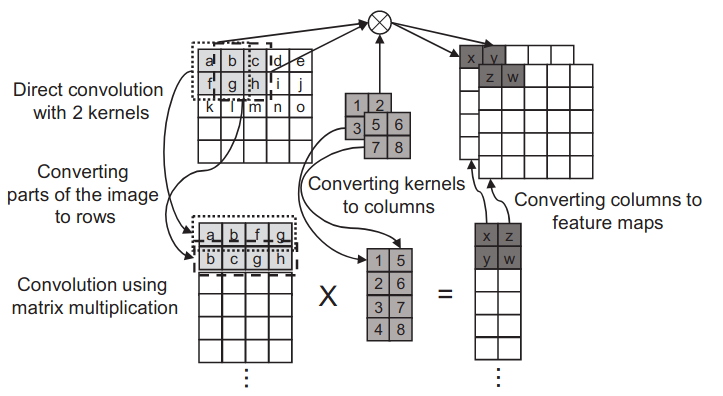
\includegraphics[width=0.9\textwidth]{assets/conv-matrix.png}
    \caption{Direct convolution is shown in the top. The transformed data and kernel for using matrix multiplication is shown in the bottom, and the arrows shows how they aretransformed. Source: \cite{perfomance_analysis_cnn}}
    \label{fig:conv_matrix}
\end{figure}

One way to optimize convolution is by using fast Fourier transform (FFT). The FFT convolution can be used to reduce the computational complexity to $O(K\times CWW \times \log W)$, which does not depend on the kernel size, however it only works with a stride of one \cite{perfomance_analysis_cnn}.
Another way to optimize the convolution operation is by using the Winograd algorithm. The Winograd algorithm is based on GEMM, it reduces multiplication operations significantly when the kernel size is fixed \cite{perfomance_analysis_cnn}. The algorithm gains performance by pre-computing matrices before using matrix multiplication. Since it needs to pre-calculate matrices it works best for small kernel sizes.

% It has been known since at least 1980 that the minimal
% filtering algorithm for computing m outputs with an $r$-tap
% FIR filter [...] requires
% $$\mu (F(m,r)) = m + r - 1$$
% multiplications \cite{fast_conv}.


\subsubsection{Dimension}%
\label{ssub:impl_dimension}

The dimension layer is a helper layer which for example makes it possible to transform the input data from one-dimensional to two-dimensional.
It works for inputs with dimensions between 1d and 3d. The layers have the following naming format \texttt{from\_\textit{x}d\_\textit{y}d} where \texttt{x} can be replaced with the input dimension and \texttt{y} can be replaced with the output dimension. For example \texttt{from\_3d\_1d}.

In the current implementation, a lot of nested \texttt{map}ping is used, however it could probably have been made more effecient by using the builtin \texttt{flatten} function.

The dimension layers are in the module \texttt{nn.dimension}.

